


\chapter{Theoretical Foundation}\label{chapter:theory}

\section{Comfort and Discomfort Definitions}

Before actually creating a metric, it is obviously crucial to have an exact definition of the terms comfort and discomfort. In this bachelor thesis comfort and discomfort will be referred to as defined by Vink et al. \cite{vink2012editorial}.

In their paper comfort is defined as "\textit{pleasant state or relaxed feeling of a human being in reaction to its environment}". Therefore comfort is a positive emotional state in reaction to the environment highly dependent on emotions and expectation. Comfort is generally related to "\textit{luxury, feeling relaxed or being refreshed}".

Discomfort on the other hand is defined as "\textit{an unpleasant state of the human body in reaction to its physical environment}". Physical stress is the main cause of discomfort, a negatively perceived state of the body. Discomfort is often felt in the form of fatigue, stiffness and pain and can in extreme cases even lead to injury.

It is important to keep in mind, that comfort and discomfort are in fact not two opposing sides on one scale. They rather are two independent factors influencing the overall well being in different ways, somewhat similar to Herzberg's motivation-hygiene theory. The absence of discomfort does not automatically result in comfort and vice versa. 

An example for the importance of this differentiation can be found when choosing the softness of foams for mattresses or seats. While softer materials will continuously increase perceived comfort, having too soft foams will result in reduced postural support, leading to higher stress on muscles and tendons and finally causing discomfort symptoms like stiffness or back pain. 

\section{Hand Comfort and Discomfort Metric Components}

Looking at the hand's anatomy the following four components were determined to be most influential on comfort and discomfort based on the definitions from above. In the following section the comfort and discomfort components will be explained and a brief idea for computation will be given. 

\subsection{Deviation from Range of Rest Posture}

The \textbf{Range of Rest Posture (RRP)} component is based on the work of Apostolico et al. \cite{apostolico2014postural}. They define the "Rest Posture" of a human joint as a posture, where involved muscles are completely relaxed or strain is minimized. When in Rest Posture, maximum comfort is perceived in that particular joint. Thus, perceived comfort should decrease when deviating from the RRP. 
Due to anatomical differences between different humans, it makes more sense to look at the so called "Range of Rest Posture", a range of angles for an articular joint, where the joint "\textit{can be considered statistically in rest}".

When looking at postures involving multiple joints, Naddeo et al. \cite{naddeo2015proposal} state that comfort can be determined by combining the comfort values of the single joints.

\begin{figure}
\centering
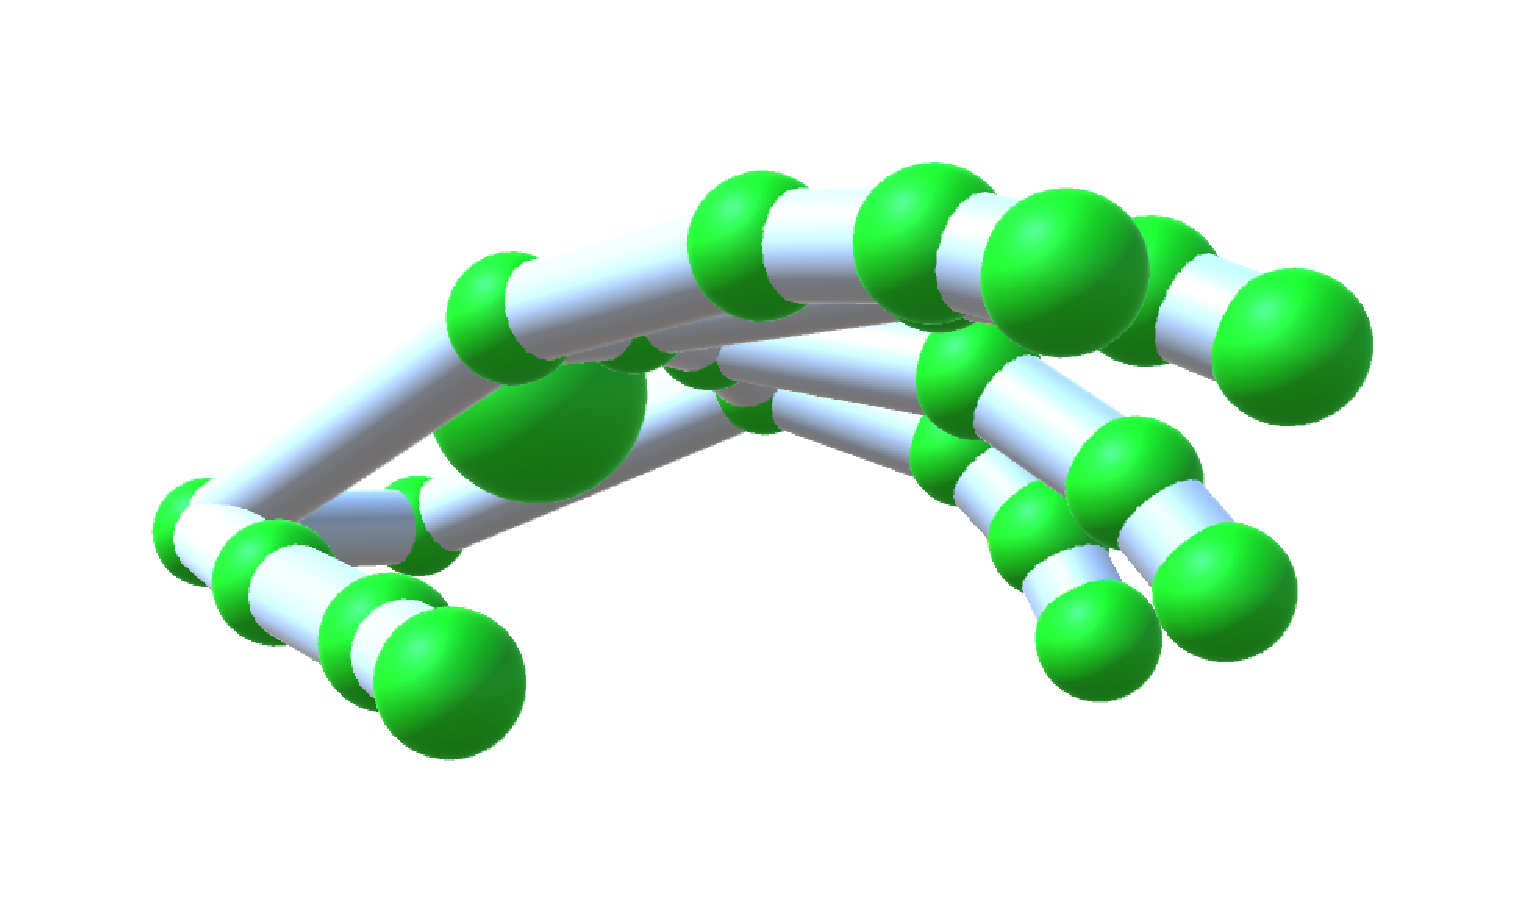
\includegraphics[width=\textwidth]{relaxed}
\caption{A relaxed Hand Posture recorded with the Leap.}
\label{fig:relaxed}
\end{figure}

In our case, we considered the human hand to have one RRP for each finger joint in a non-resting position with the palm facing downwards, resulting in a range of relaxed hand postures, similar to Figure \ref{fig:relaxed}, where the comfort is maximized. For a particular hand posture denoted by "x" the RRP component \textit{RRP(x)} can be computed by determining the angular distances to the RRP for every joint and adding them up.

\subsection{The Inter Finger Angles}

\begin{figure}
\centering
\begin{subfigure}
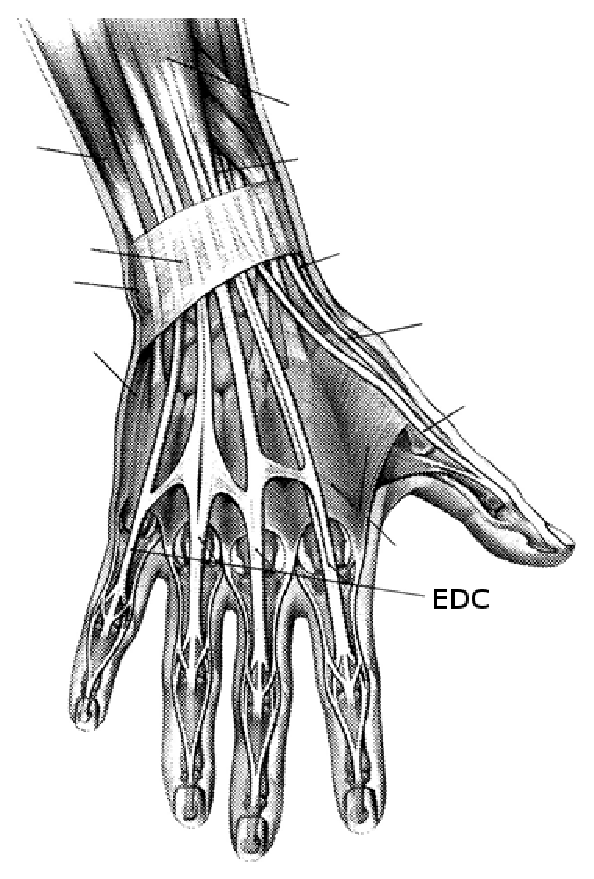
\includegraphics[width=0.4\textwidth]{Handanatomy2}
\end{subfigure}
\begin{subfigure}
\includegraphics[width=0.4\textwidth]{handanatomy}
\end{subfigure}
\caption{Hand Anatomy (from \cite{laviola1999survey})}
\label{fig:handAnatomyTotal}
\end{figure}

As it can be seen in Figure \ref{fig:handAnatomyTotal} the hand has a very compact and highly connected system of muscles, tendons and soft tissue that limits the individual movement of fingers.
The fingers, excluding the thumb, share \textbf{most} of their flexor and extendor muscles. However minor individual flexion and extension of adjacent fingers is still possible due to finger tendons originating from different areas of the muscles. In the case of the \textit{Extensor digitorum communis} (EDC in Figure \ref{fig:handAnatomyTotal}), the finger tendons are even interconnected on the back of the hand.

In addition to this, only three principal nerves serve the muscles of the hand, which makes it even harder for the motory system to fully differentiate between the individual fingers.

In conclusion of this, hand postures with high bending differences between the fingers should not only cause physical stress on both tendons and muscles, but also cognitive stress. This is due to the human trying to achieve and hold a complex posture with limited cognitive and physical means.
This can lead to severe discomfort, which is manifested in cramping up the hand and pain.
For a specific hand posture the inter finger angle component \textit{IFA(x)} can be computed, by computing the total angular flexion (Figure \ref{fig:hyperabduction}) differences of adjacent fingers and adding them up.

\subsection{Finger Hyperextension}

As highlighted by LaViola \cite{laviola1999survey} \textbf{hyperextension} (Figure \ref{fig:hyperabduction}), "\textit{puts more strain on the }[metacarpophalangeal, MCP in Figure \ref{fig:handAnatomyTotal}] \textit{joints and tendons than the hand is accustomed to}". Consequently extending the fingers beyond their natural range of motion creates noticeable amounts of discomfort. Even though this might seem redundant to the deviation from RRP on first sight, hyperextension takes a special position as it causes considerably more discomfort, compared to a full flexion of the fingers and compared to what the deviation from RRP would suggest. The hyperextension component \textit{HE(x)} can be computed by simply finding all hyperextended fingers and adding up the hyperextension angle of the MCP. 

\begin{figure}
\centering
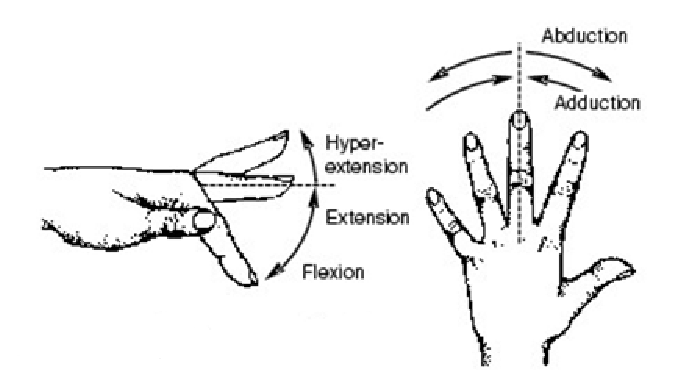
\includegraphics[width=\textwidth]{abduction}
\caption{Hyperextension and Abduction (from \cite{laviola1999survey})}
\label{fig:hyperabduction}
\end{figure}

\subsection{Finger Abduction}

Finger \textbf{abduction} (Figure \ref{fig:hyperabduction}) is the act of fanning out the fingers using the \textit{interosseus} muscles located within the hand. 
High abduction also causes stress on the MCP joints (Figure \ref{fig:handAnatomyTotal}), the muscles and tendons involved as well as the soft tissue in between the fingers.

Abduction was taken into consideration as a discomfort factor, analogue to the hyperextension, because full abduction creates substantially more discomfort than full adduction (Figure \ref{fig:hyperabduction}). By adding up all absolute abduction angles of the fingers, the finger abduction component \textit{FA(x)} can be computed.

\section{Naive Metrics}

Now that the different components most influential to comfort and discomfort are known and assumed to be computable (concrete implementation given in section \ref{chapter:handosturemetric}), it is important to think about how to combine the different factors into one metric value. 

A naive approach would be to simply sum up the single comfort and discomfort components for the whole hand. In order to compensate potential differences in intensity scales of the components, it makes sense to balance the component values with weighting coefficients \begin{math}(c_{RRP}, c_{IFA}, ...)\end{math}. The concrete weighting coefficients can be estimated and verified with experimental testing. When assigning the different components to either comfort or discomfort, following functions for a hand posture denoted by "x" can be derived.

	\[
	Comfort(x) = c_{RRP}\cdot RRP(x)
	\]
	\[
	Discomfort(x) = c_{IFA}\cdot IFA(x)  +  c_{HE}\cdot HE(x)  +  c_{FA}\cdot FA(x)
	\]
	\vspace{5pt}
	
	
The resulting metric for comfort has a minimum value of 0, where user perceived comfort is expected to be minimized. Higher metric values are due to larger distances to the RRP and therefore correspond to lower comfort values.

The discomfort metric, due to the nature of its components, also has a minimum value of 0, where user perceived discomfort is minimized. Higher amounts of discomfort are to be expected, when either high inter finger angles, hyperextension or high abduction are performed, resulting in higher discomfort metric values. 

\section{Improved Metrics}

Even though the naive metrics contain the basic causes of comfort and discomfort, they still lack deeper consideration for the anatomical differences between the fingers. The severity of this problem can be experienced when for example comparing the perceived discomfort of the standard pointing posture using the index finger to pointing with the ring finger.
The concept of improvement is straight forward: instead of applying the metrics to the whole hand, we consider the contributions from individual fingers and weight them with importance coefficients. 


	\[
	Comfort(x) = c_{RRPindex}\cdot RRP(index) + c_{RRPmiddle}\cdot RRP(middle) + ...
	\]
	\[
	Discomfort(x) = c_{IFAindex}\cdot IFA(index)  +  c_{IFAmiddle}\cdot + ... + c_{HEindex}\cdot HE(index) + ...
	\]
	\vspace{5pt}


In this context there are five comfort values and a total of twelve discomfort values, as the discomfort metric components neglect the thumb. 

However, finding the exact weighting coefficients turns out to be rather tricky, as they are generally unknown and due to their number hard to estimate. In order to solve this problem, data from a user study will be processed by a machine learning algorithm in order to compute the best fitting coefficients. In our case, the problem can be reduced to a curve fitting problem that can be solved with, for example, the least-squares algorithm.